\section{Aerial Percussion}

\paragraph{}
La percussion aérienne est un instrument de musique innovant par rapport au percussion aérienne car elle ne comporte pas les fûts qu'il faut percuter pour générer le son. La position des baguettes dans l'espace est mesurée à chaque instant grâce à des capteurs. Les données obtenues sont traitées par un logiciel qui permet de détecter les impacts en temps réel et de leur associer des sons. L'utilisation d'un ordinateur permet d'obtenir une palette sonore sans limite. Elle permet aussi au musicien de s'abstraire des contraintes physique de l'instrument, il peut chorégraphier ses mouvements, la mise en scène gagne de l'importance.
Mais comment fonctionne techniquement cette instrument?

\subsection{Polhemus Liberty}

\paragraph{}
Le Polhemus Liberty est un dispositif qui permet de connaître la position et l'orientation de capteurs dans l'espace en temps réel. Un émetteur permet de générer un champ magnétique à l'aide de trois antennes fixes placées orthogonalement les unes par rapport aux autres dans un cube d'une dizaine de centimètres de côté. Ce cube, constituant la base émettrice, est relié au bloc central par un câble et est placé idéalement au centre de la zone dans laquelle les acquisitions sont faites. Le champ magnétique diffusé est capté par un second ensemble d'antennes que constitues chacun des capteurs. Ceux-ci se présentent sous la forme de petits cubes de moins d'un centimètre de côté placés au bout des câbles qui les relient au bloc central. Le signal reçu par les capteurs est ensuite échantillonné, traité pas des processeurs DSP (Digital Signal Processor) dans le bloc central, puis envoyé à l'ordinateur via celui-ci par port USB 2.0.

Tous les composants de la percussion sont sur la figure \ref{fig:percu}, de gauche à droite il y a les baguettes, le bloc central et la base émettrice.

\begin{figure}[h!]
\centering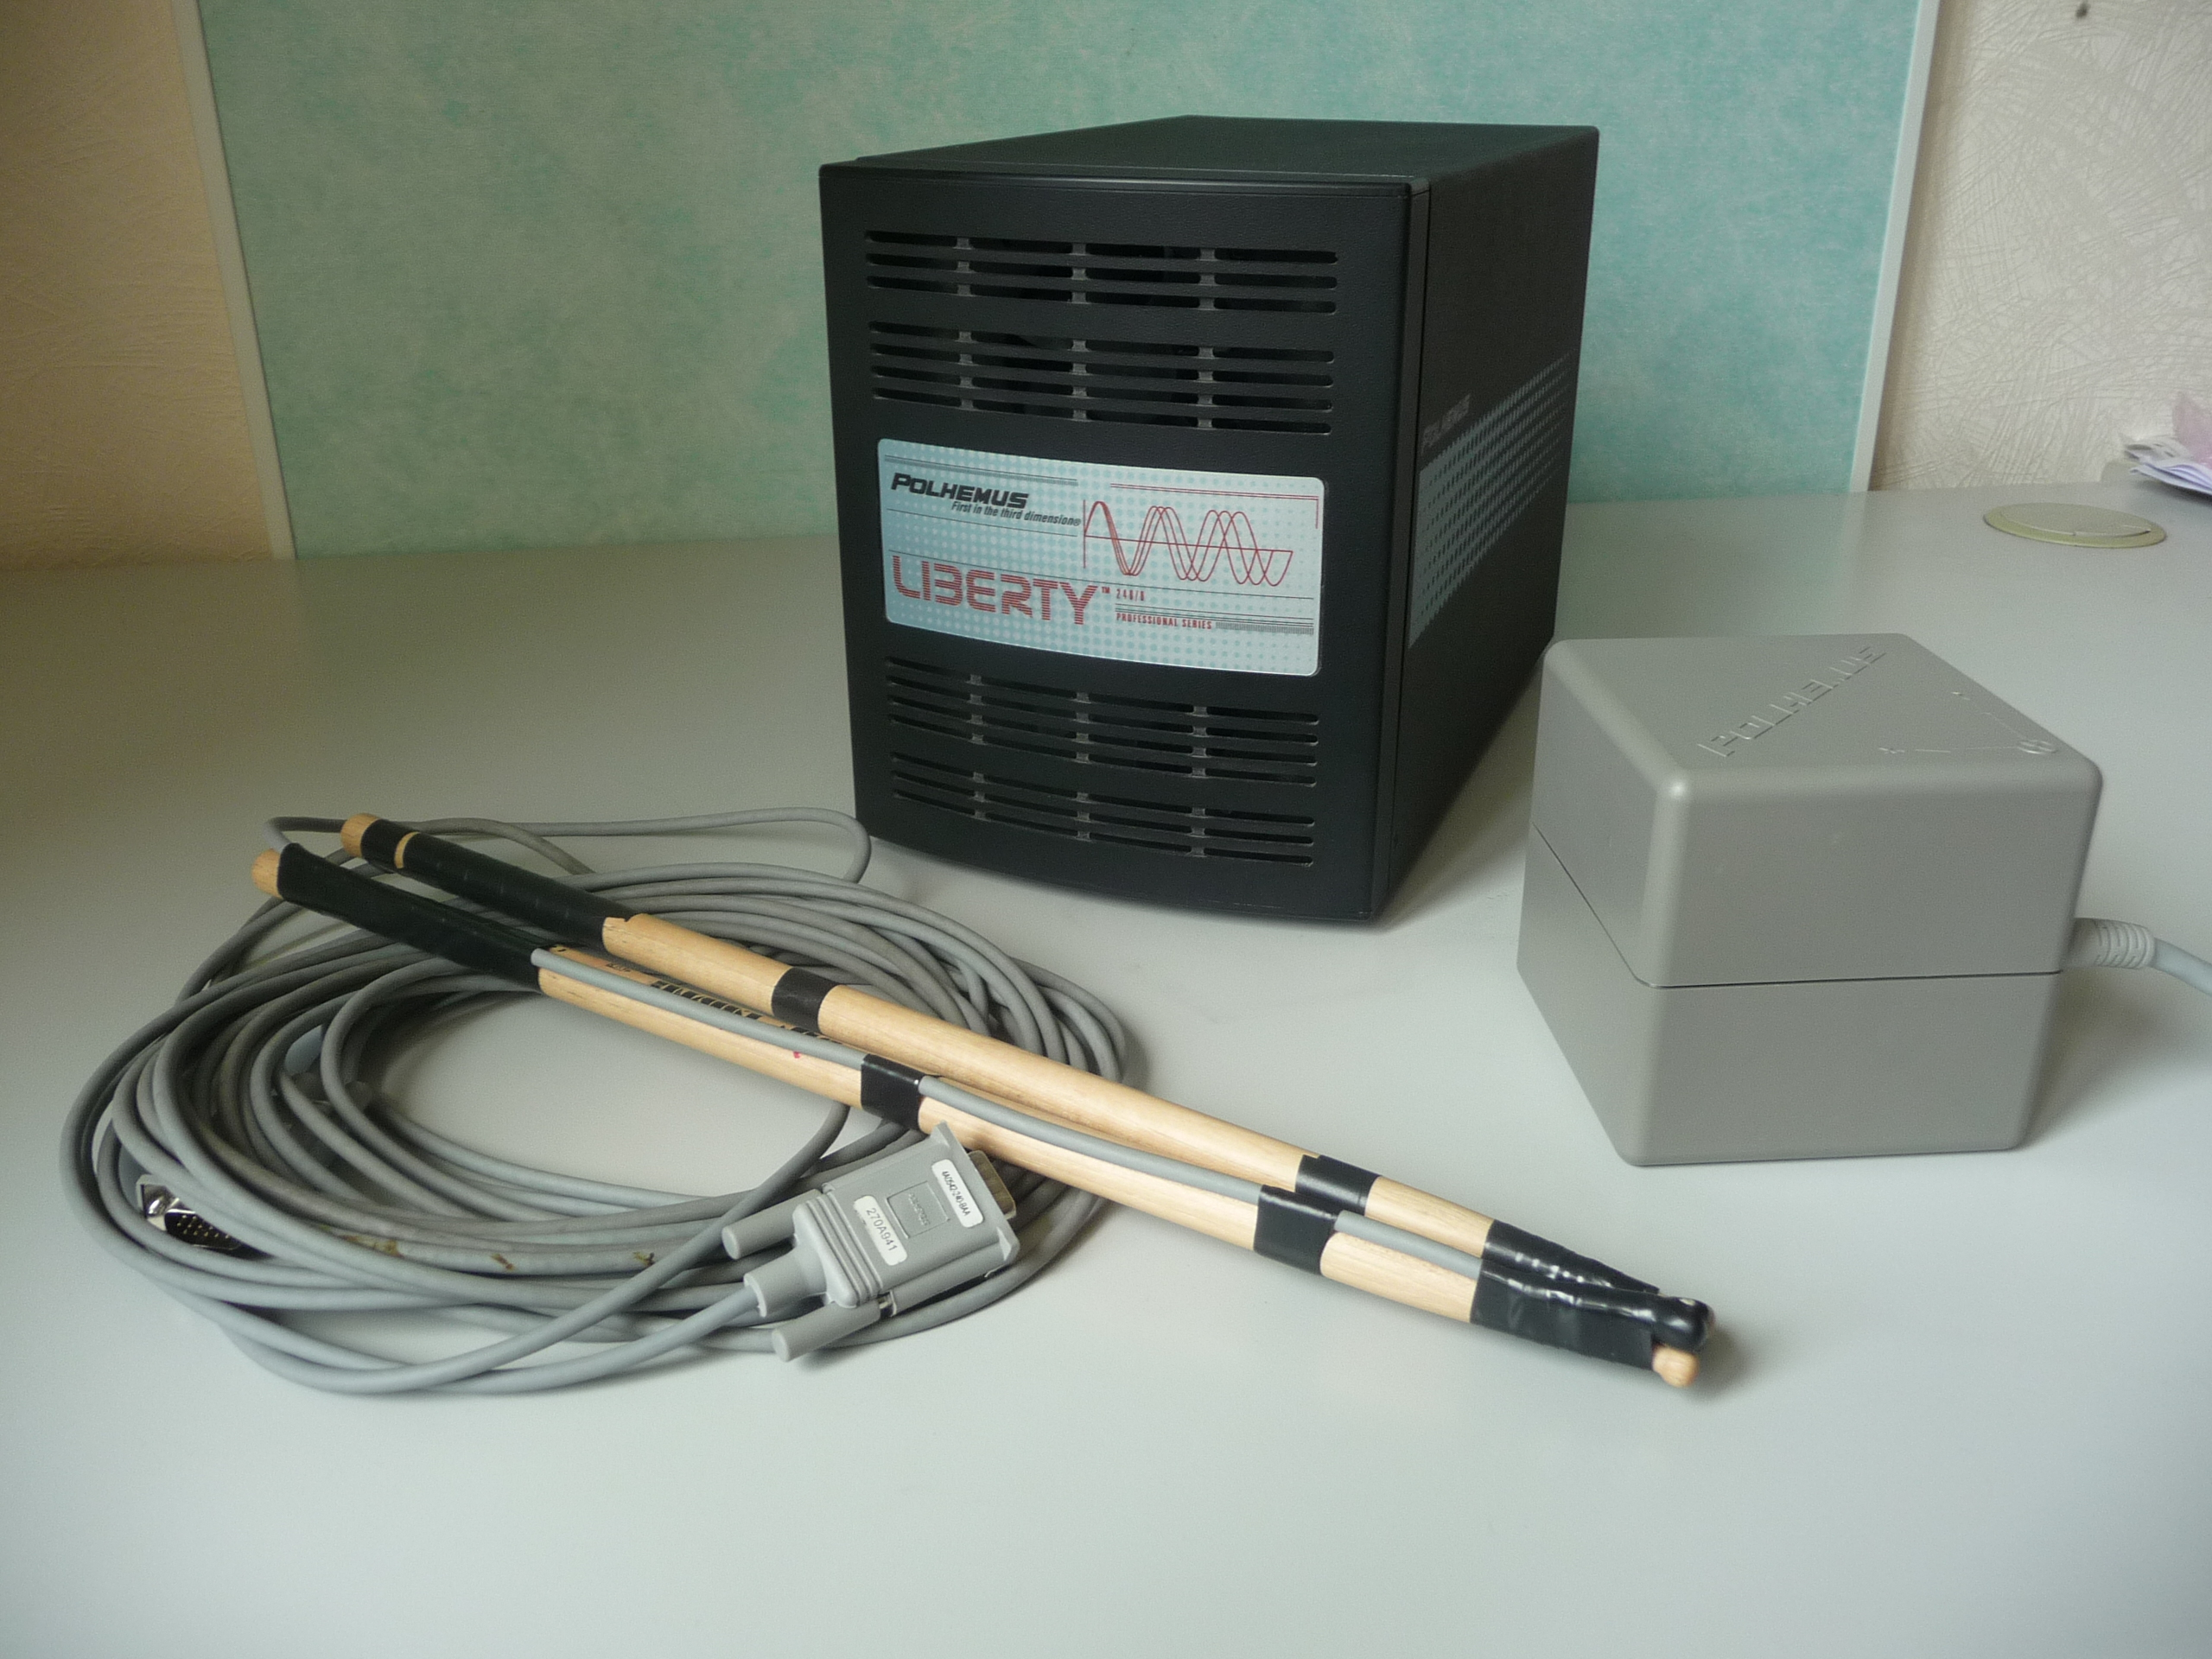
\includegraphics[scale=0.11]{image/percu.jpg}
\caption{Polhemus Liberty and sticks.}
\label{fig:percu}
\end{figure}

\paragraph{}
Mais le dispositif ne fonctionne pas seul. Il y a aussi une couche logiciel.

\subsection{SetKreator and FoB}

SetKreator a été développé au \ac{SCRIME} par Joseph Larralde et Sébastien Lebreton. SetKreator est un éditeur d'instruments virtuels pour la percussion aérienne. Il permet de créer des volumes basiques (parallépipèdes, cylindres...) à l'intérieur d'une sphère représentant la zone d'utilisation des capteurs Polhemus, comme à la figure \ref{fig:setkreator}. Il permet aussi d'associer à chaque forme une synthèse sonore particuliére. Il reçoit les données de position des baguettes par flux OSC (Open Sound Control).

\begin{figure}[h!]
\centering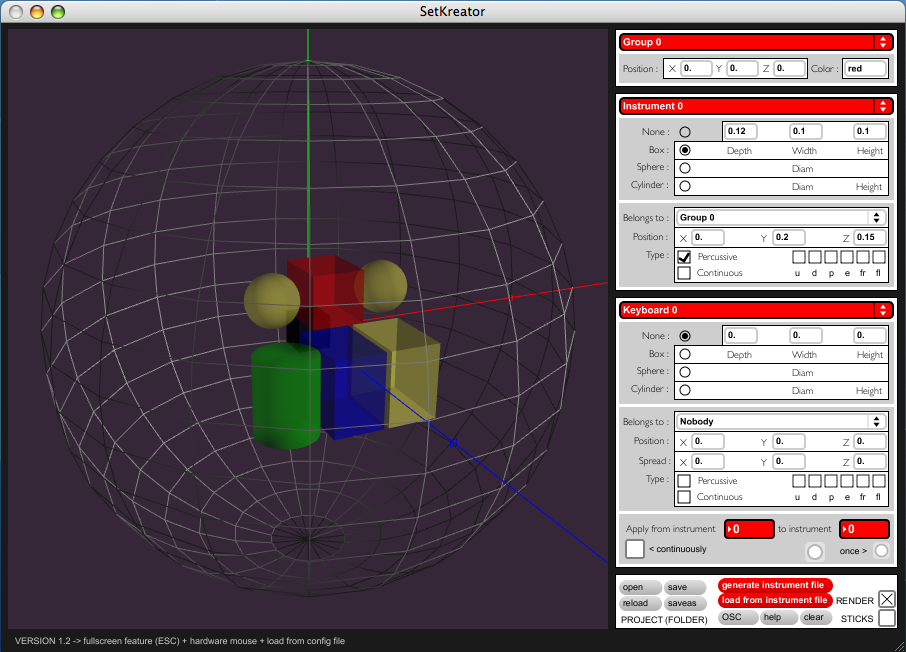
\includegraphics[scale=0.3]{image/setkreator.png}
\caption{Interface of SetKreator}
\label{fig:setkreator}
\end{figure}


Pour faire le lien entre SetKreator et le Polhemus, une autre programme est utile. Il s'agit de FoB. FoB est une petit programme qui reçoit les données de positions du Polhemus via le réseau local de l'ordinateur. Et les renvoie par flux OSC.


